\documentclass[10pt,twocolumn,letterpaper]{article}

\usepackage{cvpr}
\usepackage{times}
\usepackage{epsfig}
\usepackage{graphicx}
\usepackage{amsmath}
\usepackage{amssymb}
\usepackage{subfig}
\graphicspath{ {images/} }
% Include other packages here, before hyperref.

% If you comment hyperref and then uncomment it, you should delete
% egpaper.aux before re-running latex.  (Or just hit 'q' on the first latex
% run, let it finish, and you should be clear).
\usepackage[breaklinks=true,bookmarks=false]{hyperref}

\cvprfinalcopy % *** Uncomment this line for the final submission

\begin{document}
	
	%%%%%%%%% TITLE
	\title{Music Genre Classification}
	
	\author{Mark Gameng\\
		Illinois Institute of Technology\\
		{\tt\small mgameng1@hawk.iit.edu}
	}
	
	\maketitle
	
	\section{Introduction}
	
	Music, throughout the years, have been skyrocketing in terms of music generation and have also resulted in new styles/genres of music. Music platforms in general are producing thousands of new songs each day, with Spotify having listed over 50 million songs and over 40 thousand new songs are added every day. Years ago, the genre of songs were classified manually by people with musical knowledge. With the amount of music generation in our current era, it is imperative that music genre classification be automated through musical analysis and machine learning. Automated music genre classification will allow platforms like Spotify, Pandora, Soundcloud to better serve its customers by having a more accurate search and recommender systems. Because of this, the interest in the field of Music Information Retrieval (MIR) has been increasing ever since. Specifically, one popular topic that has garnered countless studies in MIR is music genre classification. As a result, there has also been many datasets created containing songs with information like genre.
	
	The datasets that are majorly used in these type of studies are GTZAN~\cite{tzanetakis2002musical} and Extended Ballroom~\cite{marchand2016extended}. GTZAN is the most used public dataset which consists of 1000 audio clips that are 30 seconds each and are equally classified to 10 different genres. Meanwhile, the Extended Ballroom dataset consists of 4180 audio clips that are 30 seconds each which are from 13 different ballroom genres. Other datasets to note are Free Music Archive (FMA) and Million Song which are much larger datasets with 0.1 and 1 million clips respectively.
	
	With machine learning, computer scientists have been trying to tackle the automation of music genre classification while using these datasets as a benchmark, and recently, have achieved pretty good results. A model can only learn to classify genre of music by looking at the features of it. Thus, feature extraction is one of the most important parts in music genre classification. In the past, feature extractions were done manually but currently, automatic feature extraction is done through machine learning. With just a spectrogram or any image the is able to accurately represent music, machine learning algorithms, more specifically Convolutional Neural Networks (CNN), are able to extract features and classify the genre at a very high accuracy.
	
	Previous works have tried many ways to tackle music genre classification from logistic regression up to neural networks. Notably, most high accuracy models use neural networks either on its own, or combined with another algorithm, and they all achieve in the 80\% range or higher. Specifically, a CNN~\cite{zhang2016improved}, KCNN + SVM~\cite{zhang2015deep}, and DNN~\cite{sigtia2014improved} models got 87.4\%, 83.9\%, and 83\% respectively. The best model that achieved the highest accuracy is done using a parallel recurrent convolutional neural network (PRCNN)~\cite{yang2020parallel} which got 92\% in GTZAN and 92.5\% on Extended Ballroom dataset.
	
	Most of the methods used above are trained on only one type of spectrogram, Short-time Fourier Transforms (STFT). While STFTs alone may be enough to achieve a good genre classification accuracy, combining models with different spectogram inputs may result in higher accuracies. This combination would be somewhat similar to the architecture proposed by Yang et al.~\cite{yang2020parallel} that used a CNN and a bi-directional RNN in parallel with an input of STFT. Lower end models such as logistic regression, support vector clustering/machine will probably also increase accuracy when combined with other higher end models. These are the things I will be looking at and experimenting on.
	
	\section{Data}
	
	GTZAN ~\cite{tzanetakis2002musical} dataset is widely used for music genre classification. It is a public dataset that consists of 1,000 audio clips that are 30 seconds each and are equally classified to 10 different genres. The 10 genres are blues, classical, country, disco, hiphop, jazz, metal, pop, reggae, and rock. There have been papers indicating the faults of the dataset, such as by Sturm~\cite{sturm2013gtzan}. Sturm informs that while GTZAN has its faults, it can still be used for music genre classication tasks if used with consideration of its faults.
	
	Extended Ballroom~\cite{marchand2016extended} is another dataset that is gaining popularity which is an improved version of the well-known Ballroom dataset. This dataset contains 4,180 tracks that are 30 seconds each and are classified to 13 different ballroom genres. The 13 genres are chacha, jive, quickstep, rumba, samba, tango, viennesewaltz, waltz, foxtrot, pasodoble, salsa, slowwaltz, and wcswing, Out of the 13, 10 genres have 252 to 529 tracks each while the last 3 genres only have about 50 tracks each.
	
	\subsection{Processing}
	
	GTZAN and Extended Ballroom only has 1,000 and 4,180 tracks with 10 and 13 genres respectively. GTZAN has equally distributed tracks while Extended Ballroom does not. Thus, 4 ballroom genres- Pasodoble, Salsa, Slow Waltz, Wcswing - were removed for having less than 100 tracks. This resulted in 1,000 tracks for GTZAN and 3,992 tracks for Extended Ballroom. The tracks were 30 seconds each and thus are able to be split up into shorter segments. This would allow for more data to train and test on. I opted to splitting the tracks by 10, 8, 5, 4, 2, 1 segments subsequently, which would result in more samples while also being able to test how much the time affects accuracy for music genre classification. This resulted in at max, 10,000 samples for GTZAN and 39,920 samples for Extended Ballroom. Compared to the original dataset, this amount of samples is much better and would result in the models less likely to overfit.
	
	The following features were extracted using the Python Librosa package: Short-time Fourier Transform (STFT), Mel-frequency Cepstral Coefficients (MFCC), and Melspectrogram, which are also shown in Figure ~\ref{fig:features}. Currently, STFT is the most widely used in the top accuracy models done by others. STFT simply represents a signals amplitude as it varies over time at different frequencies. MFCC are coefficients that make up an Mel-frequency spectrum (MFC) that has the frequency bands equally spaced on the mel scale which is similar to how humans perceive sounds. Somewhat similar to MFCCs, Melspectrograms are spectograms where the frequencies are converted to mel scale.
	
	\begin{figure}[!htpb]
		\centering
		\subfloat[\centering STFT]{{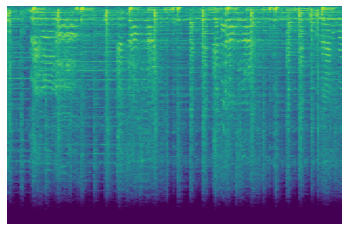
\includegraphics[width = 3cm]{STFT.png}}}
		\qquad
		\subfloat[\centering MFCC]{{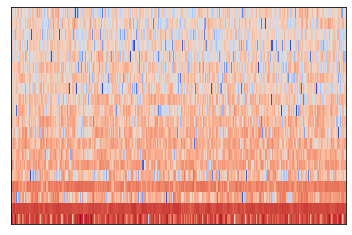
\includegraphics[width = 3cm]{MFCC.png}}}
		
		\subfloat[\centering Melspectrogram]{{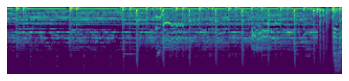
\includegraphics[width = 5cm]{MELSPECTROGRAM.png}}}
		\caption{Feature Extraction from Audio}
		\label{fig:features}
	\end{figure}
	
	\section{Methodology}
	
	Due to the low amount of samples in both GTZAN and Extended Ballroom dataset, splitting the samples into multiple segments would be beneficial in terms of accuracy and generalization. The tracks were split into 10, 8, 5, 4, 2, 1 segments with no overlap. Thus the samples ranged from 3 seconds to 30 seconds of audio. With a split of 10 segments for each sample, GTZAN now has 10,000 samples and Extended Ballroom with 39,920. 
	
	For model training, 20\% of samples were set aside for testing. This resulted in 80\% of the samples being used for training, in which 20\% of that is used for validation. Thus, it is a 64-16-20 split for training, validation, and testing. Aside from sample splitting, other methods were used such as early stopping, regularization, and dropouts for neural networks to avoid overfitting. While training, the best model is determined and used using the least validation loss through model checkpoints. The following sections describe the methods and architectures used. Currently, I have only done CNN as I have yet to do RNN, SVM and other stuff.
	
	\subsection{CNN}
	
	Due to the different shapes of the spectrograms for the input, the models for each feature vary a little from each other, however the general structure is the same. The spectograms has the shapes (1025, 64), (20, 64), (64, 64) with 10 splits for STFT, MFCC, and Melspectrogram respectively. As a result for the smaller shapes, I decided to use 4 convolutional layers for MFCC and Melspectrogram while using 5 for STFT. After each convolutional layer, a max pooling operation and dropout is done to overall reduce overfitting and extract only the most needed music features. The convolutional layers all have padding, kernel size of (3, 3), and strides of (1, 1) with rectified linear units (ReLUs) activation function. The filters for STFT are (16, 32, 64, 128, 64) and for MFCC and Melspectrogram, (32, 64, 128, 64). For the max pooling operation, pool size is (2, 2) and strides is (2, 2). For each convolutional layer the dropout is 0.25.
	
	After it has gone through all the convolutional layers, the output is flattened and a 0.5 dropout is once again used. The output is then fed to a dense layer of 256 neurons and a ReLU activation with l2 regularization. Afterwards, a 0.25 dropout is used, and then the final dense layer of \#genres neurons with softmax activation to classify the music genres.
	
	\subsection{To Do}
	
	I have yet to form and test RNN architectures and combining models together to achieve higher accuracies. RNN would be useful and I think more successful than CNN because they can extract temporal information from the spectrogram. For the parallel/combination of models, I will be trying same input as well as different feature inputs and see which works best. I may also combine using classical methods such as logistic regression, random forest, SVMs, etc. After optimizing, I will also be using majority voting since the clips were split into segments and seeing if it results in better accuracies.
	
	\section{Results}
	
	The models specified in the previous section were trained using the GTZAN and Extended Ballroom dataset and the results from each of the different models are shown in Table ~\ref{table:resultsGTZAN} and ~\ref{table:resultsExtendedBallroom}, for GTZAN and Extended Ballroom respectively. Only the top models are shown, with the accuracy of other models included for comparison. Due to utilizing different features and optimization, the general structure of the models are similar, but not one to one. Only the best models of each type are thoroughly described in the methodology section.
	
	The following models on each of the tables are using the 8 split segmented audios which are about 3.75 seconds each. Those segments are the best in terms of accuracy and generalization.
	
	\begin{table}[!htbp] % !htbp for table positioned correctly according to text layout here
	\caption{Results on GTZAN}
	\centering
		\resizebox{\columnwidth}{!}{
		\begin{tabular}[b]{ccc}
			\hline \hline
			Model & Feature & Accuracy 	\\ [0.5ex]
			\hline
			MusicRecNet + SVM ~\cite{elbir2020music} & Melspectrogram & 97.6\%			\\
			\textbf{Dual CNN + KNN} & \textbf{STFT, Melspectrogram} & \textbf{95.8\%} 			\\
			\textbf{Dual CNN + KNN} & \textbf{STFT, MFCC} & \textbf{95.3\%} 			\\
			\textbf{Dual CNN + SVM} & \textbf{STFT, MFCC} & \textbf{94.0\%} 			\\
			Broadcast NN ~\cite{liu2020bottom} & Melspectrogram & 93.9\%			\\
			CNN + 1-layer RNN~\cite{yang2020parallel} & STFT & 90.2\%			\\
			CNN + 2-layer RNN~\cite{yang2020parallel} & STFT & 88.8\%			\\
			CNN~\cite{yang2020parallel} & STFT & 88.0\%							\\
			\textbf{CNN} & \textbf{STFT} & \textbf{86.3\%} 					\\
			\textbf{CNN} & \textbf{Melspectrogram} & \textbf{84.0\%} 			\\
			2-layer BRNN~\cite{schuster1997bidirectional} & STFT & 76.2\% 		\\
			\textbf{CNN} & \textbf{MFCC} & \textbf{70.1\%} 			\\[1ex]
			\hline \hline
		\end{tabular}}
	\label{table:resultsGTZAN}
	\end{table}\textsc{}

	In terms of the GTZAN dataset, the models described in the previous section resulted in respectable accuracies compared to others. A simple 5 and 4 layer CNN model using STFT and Melspectogram achieved 86.2\% and 83.1\% respectively. Those models are what I currently have done and I have not even tried optimizing them yet. After optimizing them, I will be combining them with each other and other models, similar to the model made by Yang et al.~\cite{yang2020parallel}, however with different feature inputs. The resulting models will be placed in Table ~\ref{table:resultsGTZAN} as well.
	
	\begin{table}[!htbp] % !htbp for table positioned correctly according to text layout here
		\caption{Results on Extended Ballroom}
		\centering
		\resizebox{\columnwidth}{!}{
		\begin{tabular}[b]{ccc}
			\hline \hline
			Model & Feature & Accuracy 	\\ [0.5ex]
			\hline
			Broadcast NN ~\cite{liu2020bottom} & Melspectrogram & 97.2\%			\\
			CNN + 2-layer RNN~\cite{yang2020parallel} & STFT & 92.5\%			\\
			\textbf{Dual CNN + SVM} & \textbf{STFT, MFCC} & \textbf{92.4\%} 			\\
			CNN + 1-layer RNN~\cite{yang2020parallel} & STFT & 92.3\%			\\
			CNN~\cite{yang2020parallel} & STFT & 92.2\%							\\
			\textbf{Dual CNN + RF} & \textbf{STFT, MFCC} & \textbf{91.9\%} 			\\
			\textbf{Dual CNN + SVM} & \textbf{STFT, Melspectrogram} & \textbf{91.9\%} 			\\
			2-layer BRNN~\cite{schuster1997bidirectional} & STFT & 90.3\% 		\\
			\textbf{CNN} & \textbf{STFT} & \textbf{90.3\%} 			\\
			\textbf{CNN} & \textbf{Melspectrogram} & \textbf{87.0\%} 	\\
			\textbf{CNN} & \textbf{MFCC} & \textbf{81.5\%} 			\\[1ex]
			\hline \hline
		\end{tabular}}
	\label{table:resultsExtendedBallroom}
	\end{table}

	In terms of the Extended Ballroom dataset, the models described in the previous section resulted in respectable but lower accuracies compared to other models tested in the same dataset. I haven't spent time optimizing the models, so the accuracies might still increase and be more similar or better than other models. I will also be combining them together or with other models to try and achieve even better accuracies. The resulting models will be placed in Table ~\ref{table:resultsExtendedBallroom} as well.
	
	Currently, I have only trained CNN models that I think results in the best accuracy. Thus, the results don't include all the possible models with splits and features. However, the current results are already promising, with the models having at least 80\% accuracy. With optimization and added features such as majority voting or using models together, the accuracy can still be increased. I also intend on training the models multiple times to instead show the average accuracy rate, which, I think, is more representative. 
	
	Using multiple splits to train will be helpful in determining up to what length of audio can a model accurate classify the genre. Doing so will allow me to choose the best model based on effectiveness and efficiency. The results for each split and models are shown in Table ~\ref{table:splitsGTZAN} and ~\ref{table:splitsExtendedBallroom}, for GTZAN and Extended Ballroom respectively.
	
	% These tables of STFT, gram, MFCC splits should be after conclusion. Cuz lots of data, not really essential, just the best one
	\begin{table}[!htbp] % !htbp for table positioned correctly according to text layout here
		\caption{Impact of Splits in GTZAN}
		\centering
		\resizebox{\columnwidth}{!}{
		\begin{tabular}[b]{cccc}
			\hline \hline
			Model & Feature & Split & Accuracy 		\\ [0.5ex]
			\hline
			CNN & STFT &  10 & 82.5\%				\\
			CNN & STFT &  8 & 86.3\%				\\
			CNN & STFT &  4 & 86.3\%				\\
			CNN & STFT &  1 & 57.0\%				\\
			CNN & MFCC &  1 & 60.0\%				\\
			CNN & MFCC &  4 & 67.0\%				\\
			CNN & MFCC &  8 & 70.1\%				\\
			CNN & MFCC &  10 & 75.9\%				\\
			CNN & Melspectrogram & 10 & 83.3\% 		\\
			CNN & Melspectrogram & 8 & 84.0\% 		\\
			CNN & Melspectrogram & 4 & 83.7\% 		\\
			CNN & Melspectrogram & 1 & 71.5\% 		\\ [1ex]
			\hline \hline
		\end{tabular}}
	\label{table:splitsGTZAN}
	\end{table}

	\begin{table}[!htbp] % !htbp for table positioned correctly according to text layout here
		\caption{Impact of Splits in Extended Ballroom}
		\centering
		\resizebox{\columnwidth}{!}{
		\begin{tabular}[b]{cccc}
			\hline \hline
			Model & Feature & Split & Accuracy 		\\ [0.5ex]
			\hline
			CNN & STFT &  10 & 89.4\%				\\
			CNN & STFT &  8 & 90.3\%				\\
			CNN & STFT &  4 & 91.3\%				\\
			CNN & STFT &  1 & 92.6\%				\\
			CNN & MFCC &  10 & 80.5\%				\\
			CNN & MFCC &  8 & 81.5\%				\\
			CNN & MFCC &  4 & 83.4\%				\\
			CNN & MFCC &  1 & 41.8\%				\\
			CNN & Melspectrogram & 10 & 85.0\% 		\\
			CNN & Melspectrogram & 8 & 87.0\% 		\\
			CNN & Melspectrogram & 4 & 90.4\% 		\\
			CNN & Melspectrogram & 1 & 91.4\% 		\\ [1ex]
			\hline \hline
		\end{tabular}}
	\label{table:splitsExtendedBallroom}
	\end{table}
	
	
	
		
	{\small
		\bibliographystyle{ieee_fullname}
		\bibliography{egbib}
	}
	
\end{document}